\subsection{ゲーム画面}
初期画面を図\ref{gamescreen}に示す.
ゲームを開始すると同時にテトリミノが落下を始める.
\subsection{テトリミノの落下}
テトリミノの落下を図\ref{fool}に示す.
テトリミノは,毎秒1ブロックの速さで落下する.
\subsection{テトリミノの固定}
テトリミノの固定を図\ref{stick}に示す.
テトリミノは,他のブロックや下の範囲に触れると固定される.
\subsection{テトリミノの新規作成}
テトリミノの新規作成を図\ref{new}に示す.
テトリミノが固定されると新しく操作可能なブロックが作成される.
\subsection{1行消去のスコア加算}
1行消去したときのスコア加算を図\ref{one1},\ref{one2}に示す.
1行消去されるとスコアが100加算される.
\subsection{2行消去のスコア加算}
2行消去したときのスコア加算を図\ref{two1},\ref{two2}に示す.
2行消去されるとスコアが100加算される.
\subsection{3行消去のスコア加算}
3行消去したときのスコア加算を図\ref{three1},\ref{three2}に示す.
3行消去されるとスコアが100加算される.
\subsection{4行消去のスコア加算}
4行消去したときのスコア加算を図\ref{tetoris}に示す.
4行消去されるとスコアが100加算される.
\subsection{ゲームオーバー画面}
ゲームオーバー画面を図\ref{gameover}に示す.
ブロックが新しく出たときに操作不可能だった場合固定される.

\begin{figure}[htb]
  \begin{center}
    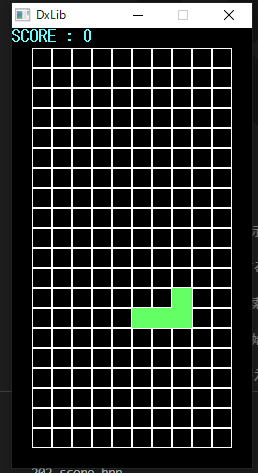
\includegraphics[scale=0.5]{./soft_img/gamescreen.png}
    \caption{ゲーム画面}
    \label{gamescreen}
  \end{center}
\end{figure}
\begin{figure}[htb]
  \begin{center}
    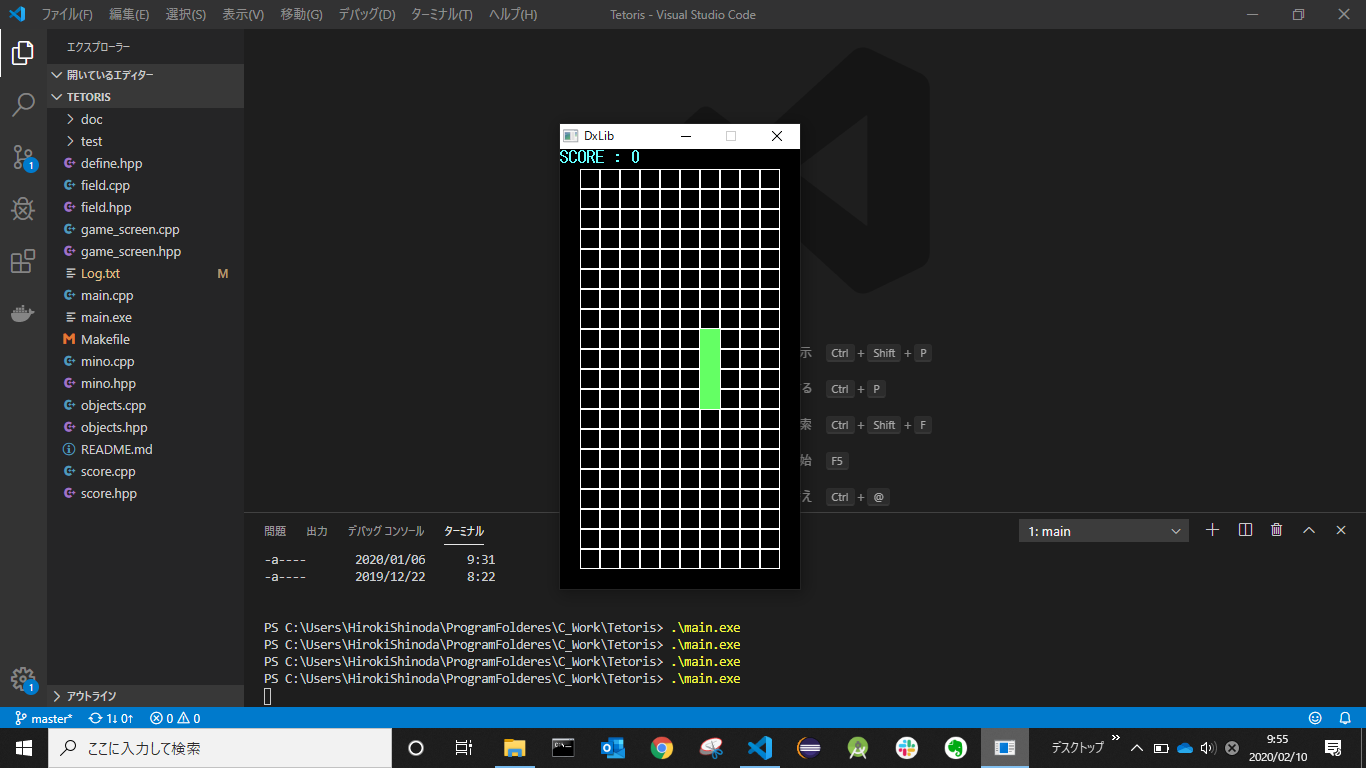
\includegraphics[scale=0.5]{./soft_img/fall.png}
    \caption{テトリミノの落下}
    \label{fool}
  \end{center}
\end{figure}
\begin{figure}[htb]
  \begin{center}
    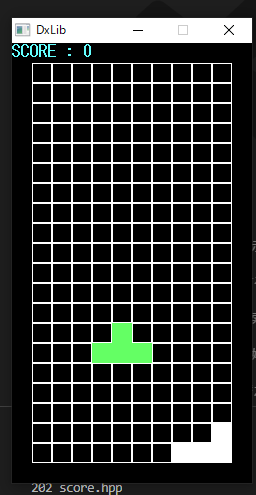
\includegraphics[scale=0.5]{./soft_img/stick.png}
    \caption{テトリミノの固定}
    \label{stick}
  \end{center}
\end{figure}
\begin{figure}[htb]
  \begin{center}
    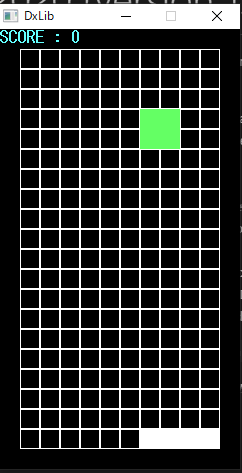
\includegraphics[scale=0.5]{./soft_img/newblock.png}
    \caption{テトリミノの新規作成}
    \label{new}
  \end{center}
\end{figure}
\begin{figure}[htb]
  \begin{center}
    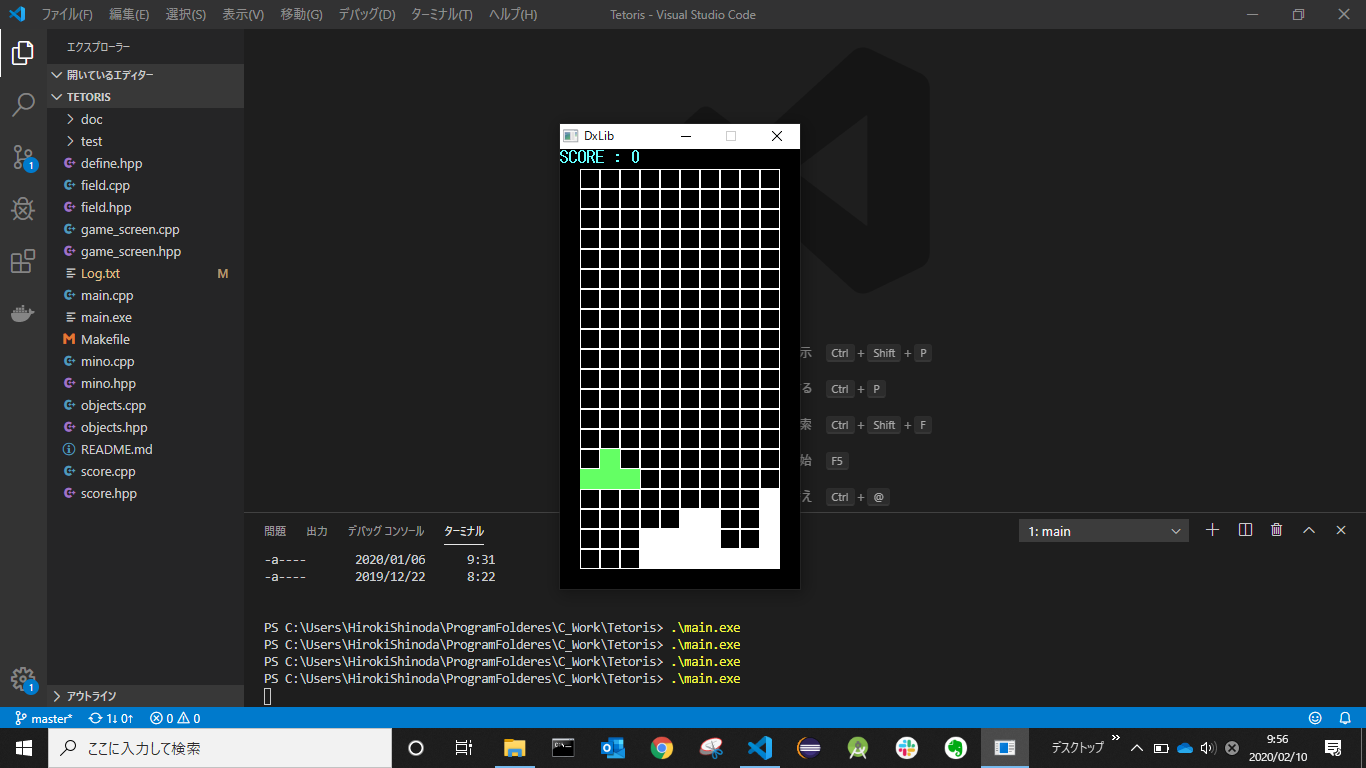
\includegraphics[scale=0.5]{./soft_img/onelinebefore.png}
    \caption{1行消去前の画面}
    \label{one1}
  \end{center}
\end{figure}
\begin{figure}[htb]
  \begin{center}
    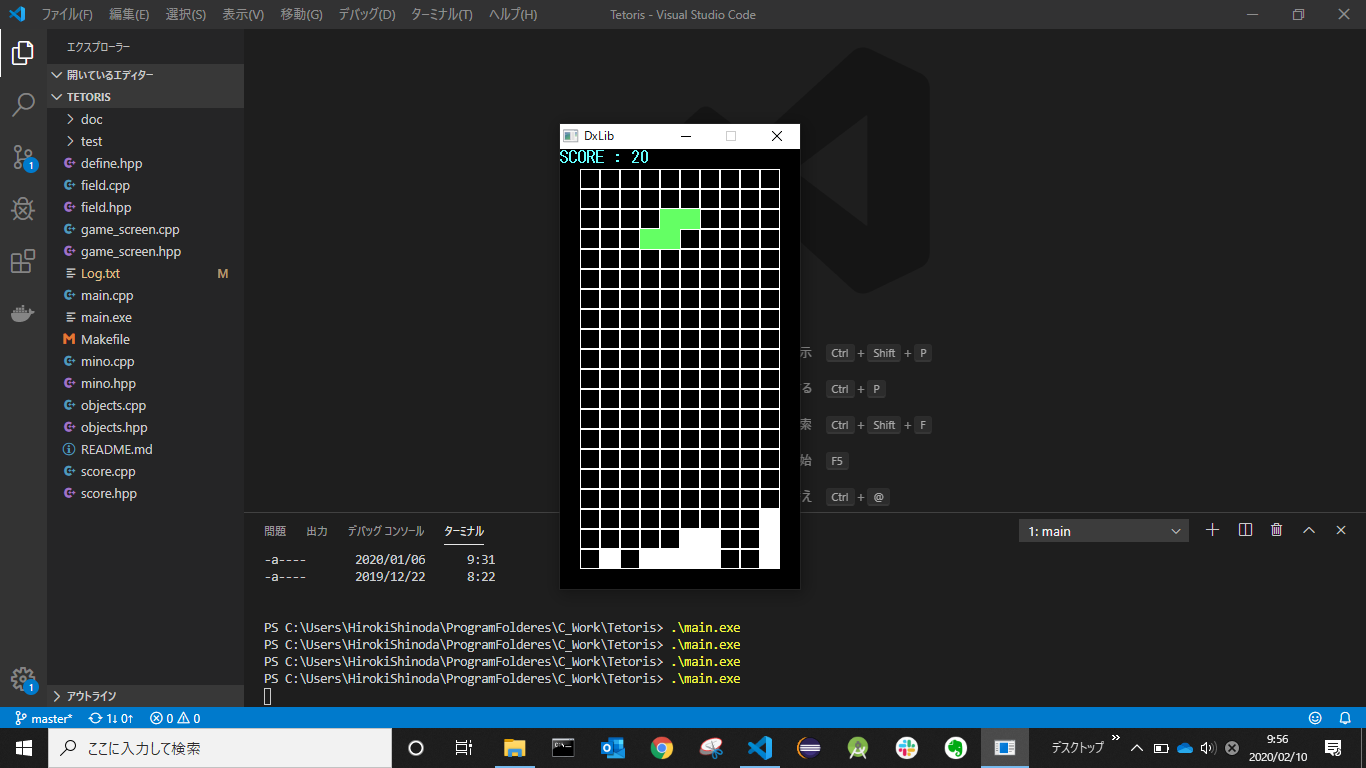
\includegraphics[scale=0.5]{./soft_img/onelineafter.png}
    \caption{1行消去後の画面}
    \label{one2}
  \end{center}
\end{figure}
\begin{figure}[htb]
  \begin{center}
    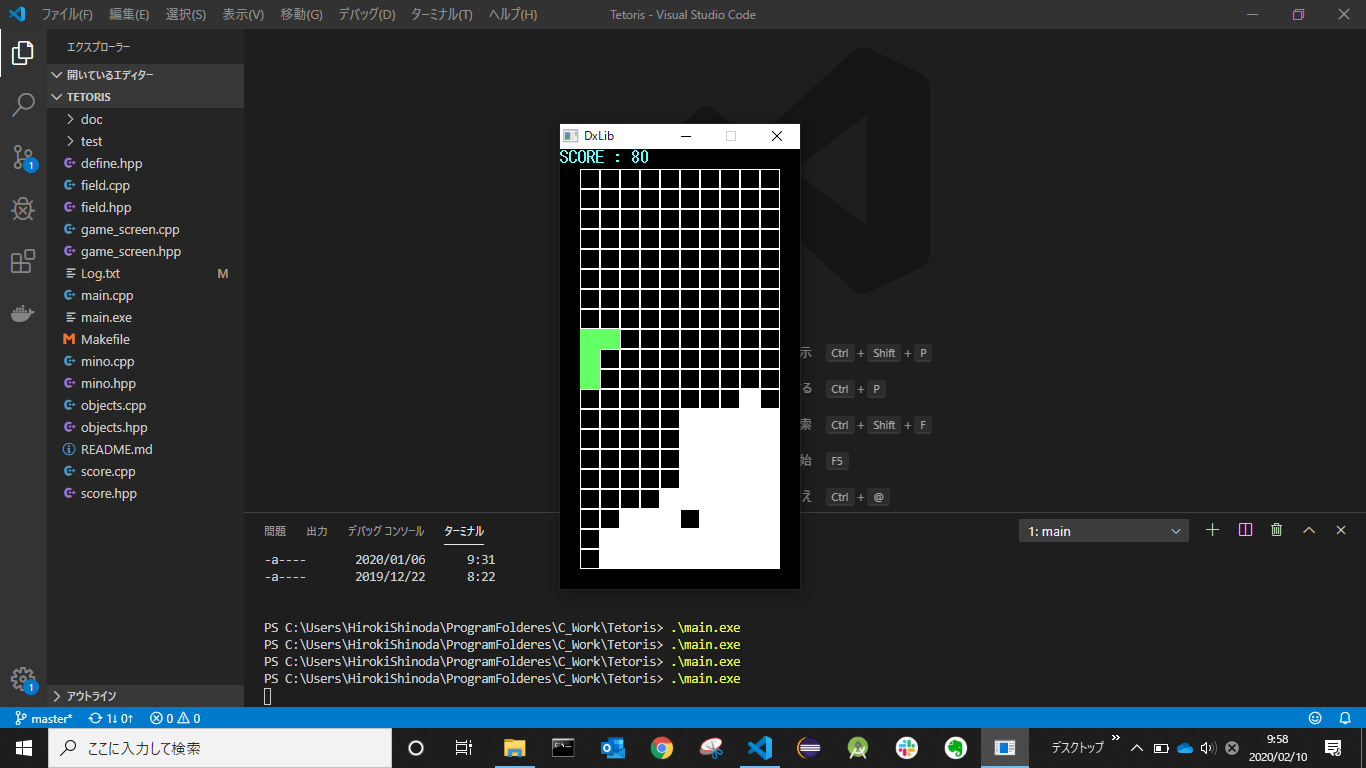
\includegraphics[scale=0.5]{./soft_img/twolinebefore.png}
    \caption{2行消去前の画面}
    \label{two1}
  \end{center}
\end{figure}
\begin{figure}[htb]
  \begin{center}
    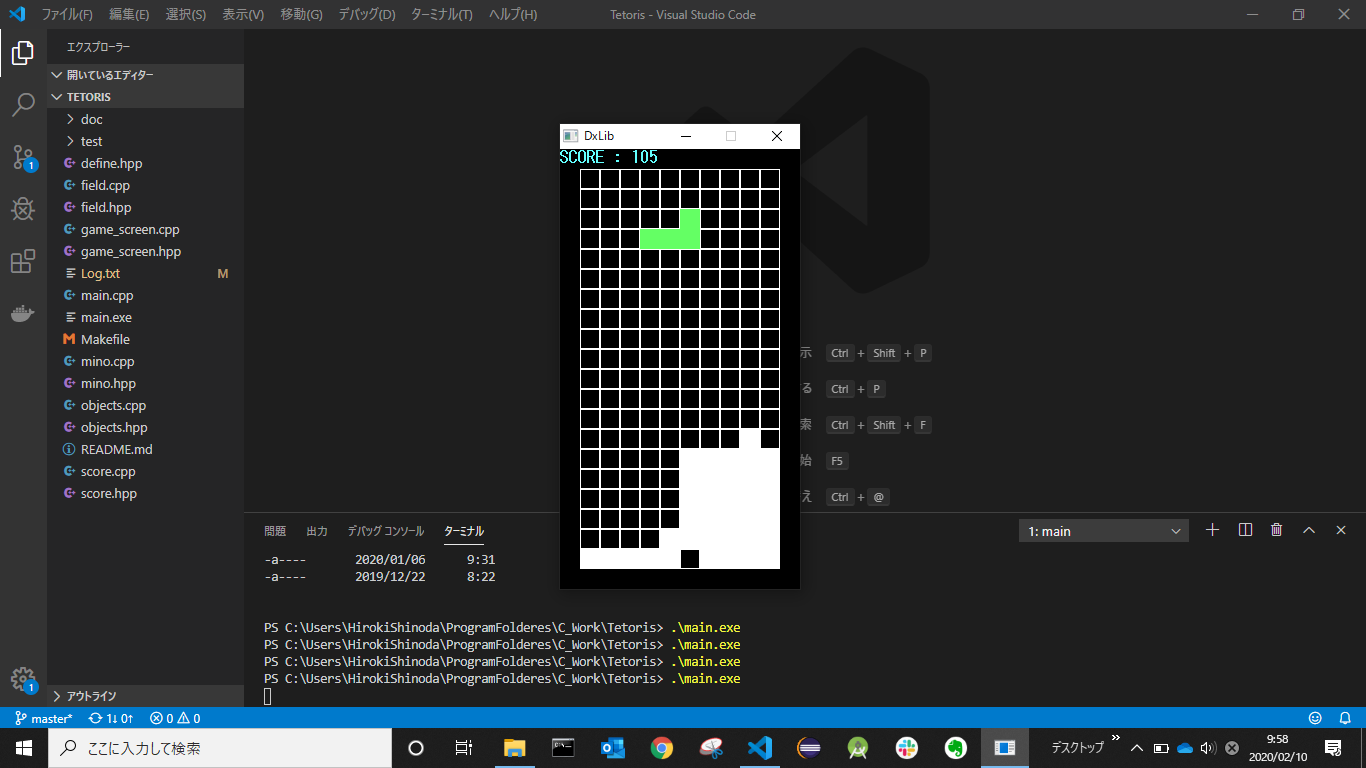
\includegraphics[scale=0.5]{./soft_img/twolineafter.png}
    \caption{2行消去後の画面}
    \label{two2}
  \end{center}
\end{figure}
\begin{figure}[htb]
  \begin{center}
    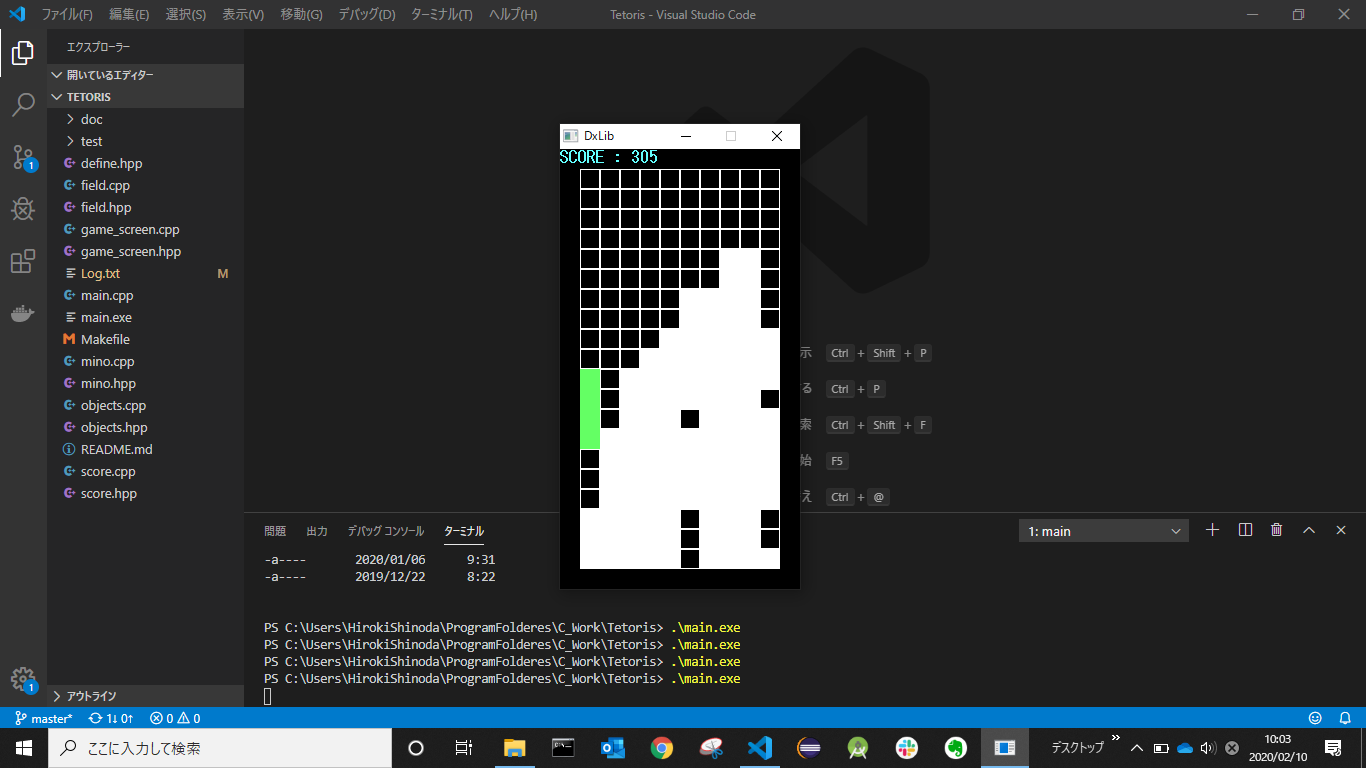
\includegraphics[scale=0.5]{./soft_img/threelinebefore.png}
    \caption{3行消去前の画面}
    \label{three1}
  \end{center}
\end{figure}
\begin{figure}[htb]
  \begin{center}
    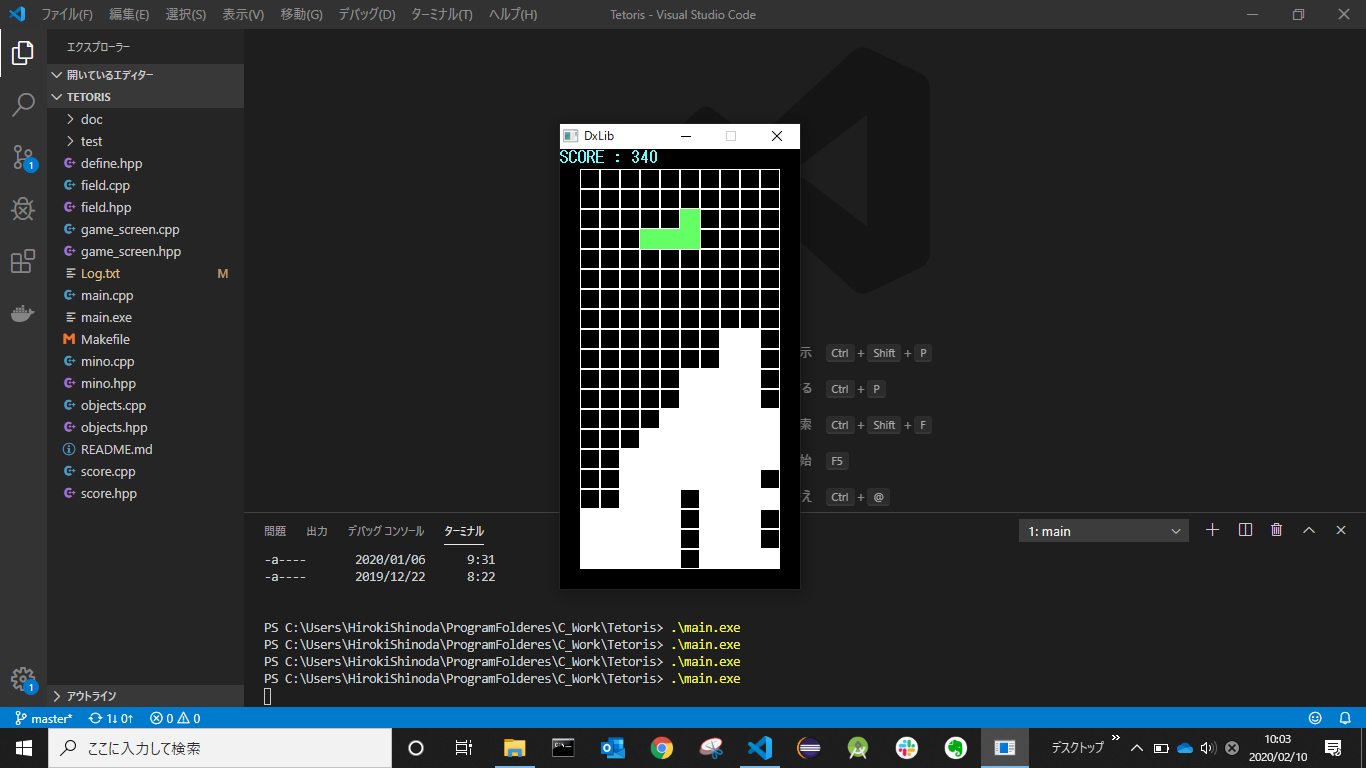
\includegraphics[scale=0.5]{./soft_img/threelineafter.png}
    \caption{3行消去後の画面}
    \label{three2}
  \end{center}
\end{figure}
\begin{figure}[htb]
  \begin{center}
    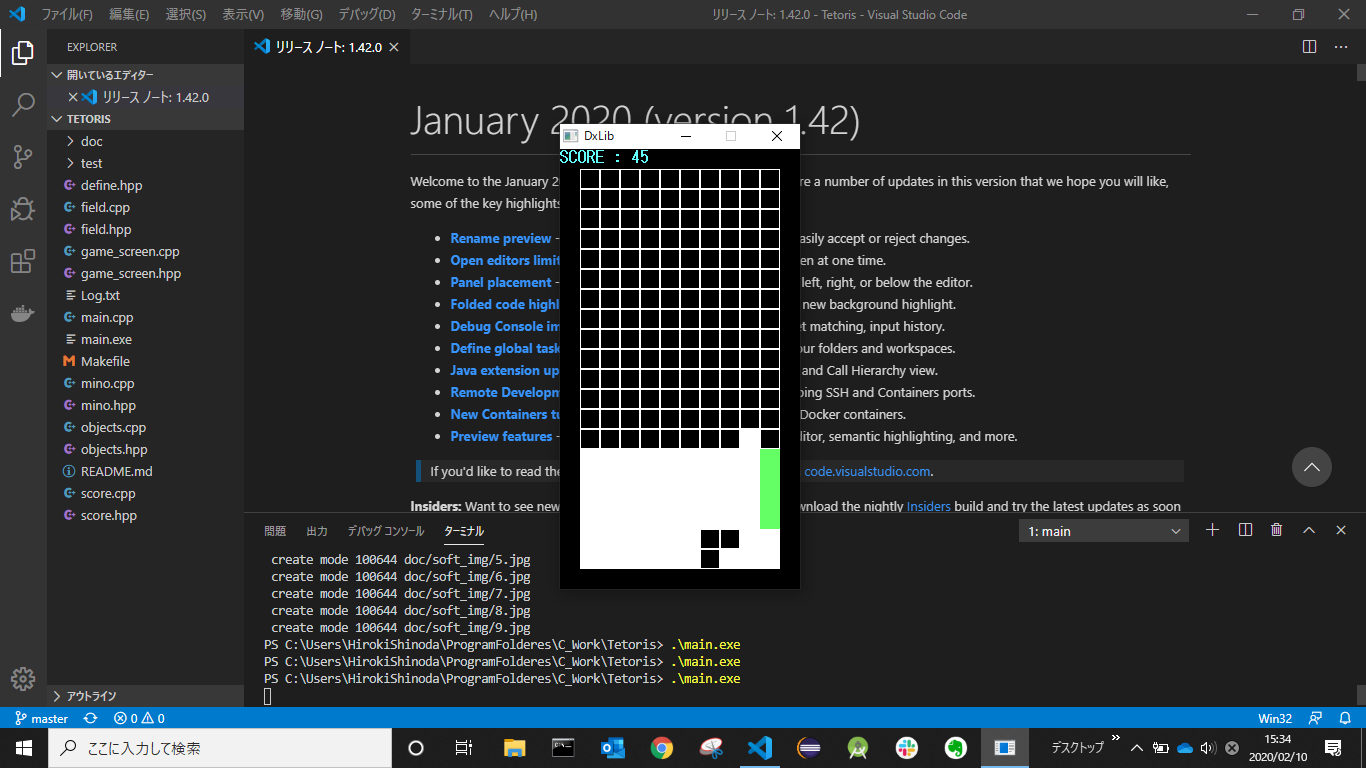
\includegraphics[scale=0.5]{./soft_img/tetoris.png}
    \caption{4行消去の画面}
    \label{tetoris}
  \end{center}
\end{figure}
\begin{figure}[htb]
  \begin{center}
    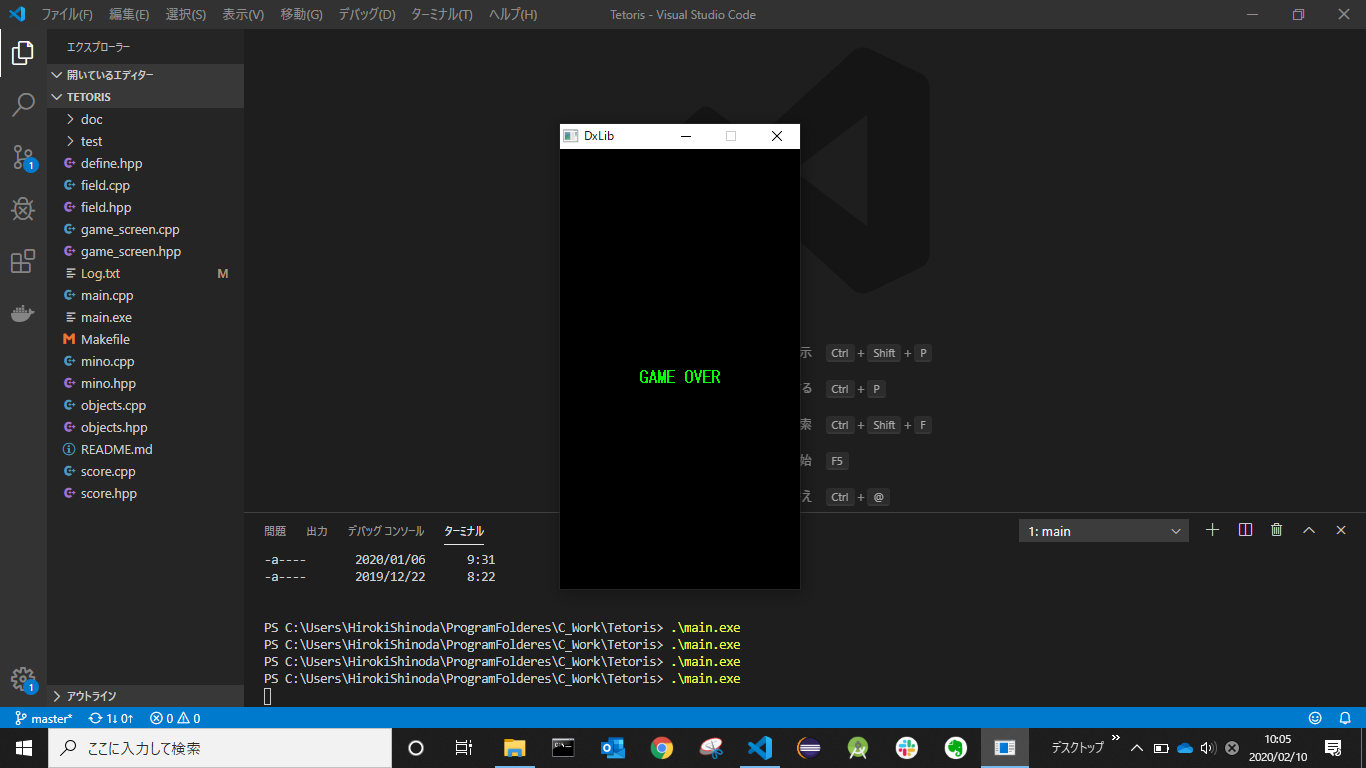
\includegraphics[scale=0.5]{./soft_img/gameover.png}
    \caption{ゲームオーバー画面}
    \label{gameover}
  \end{center}
\end{figure}
